%%%%%%%%%%%%%%%%%%%%%%%%%%%%%%%%%%%%%%%%%%%%%%%%%%%%%%%%%%%%%%%%%%%%%%
% LatexTemplate
% November 10, 2012
% By Simon Pratt (mostly)
\documentclass[11pt]{article}

\usepackage{Assignment}
\usepackage{CGAlgorithms}
\usepackage{QuestionAnswer}
\usepackage{TheoremStuff}
\usepackage{HeaderStuff}
\usepackage{url}
\usepackage{hyperref}
\usepackage{nonfloat}

%%%%%%%%%%%%%%%%%%%%%%%%%%%%%%%%%%%%%%%%%%%%%%%%%%%%%%%%%%%%%%%%%%%%%%
% Multicolumn stuff
\usepackage{multicol}
\usepackage{newclude} % \include without \clearpage

%%%%%%%%%%%%%%%%%%%%%%%%%%%%%%%%%%%%%%%%%%%%%%%%%%%%%%%%%%%%%%%%%%%%%%
% Configuration
\fancyhead[L]{COMP4106 - Final Project}
\fancyhead[R]{Simon Pratt - 100663987}
\bibliographystyle{plain}

%%%%%%%%%%%%%%%%%%%%%%%%%%%%%%%%%%%%%%%%%%%%%%%%%%%%%%%%%%%%%%%%%%%%%%
% Document
\begin{document}
\begin{multicols}{2} % remove line if you don't want multiple columns

% Content starts here

\section{The Problem}

The problem herein considered is that of Frequent Pattern Mining.
Given a large dataset of transactions each containing several items,
find sets of a given cardinality containing items which occur together
frequently.  Frequently being that the number of transactions in which
the items occur together (their ``support'') is more than some
minimum.

\subsection{Motivation}

Frequent patterns in data can give us insight into the semantic
meaning of the data.  In particular, if we are mining for frequent
patterns in a data set of actions we can identify typical workflow and
anomalous activity, which could be useful for security or process
optimization.

\section{Algorithms}

I implemented the following algorithms for mining frequent patterns:
\texttt{Apriori}, \texttt{FP-growth}, and \texttt{Eclat}
\cite{Han2007,fpmlecture}.

\subsection{Apriori}

This algorithm is based on the antimonotone property of frequent
itemsets.  That is to say, subsets of frequent itemsets must
themselves be frequent itemsets.  With this in mind, to find frequent
itemsets of size k, we begin by finding all frequent itemsets of size
1, which simply means to count the occurences (called the support) of
each item in the dataset.  For efficiency, we may also set a minimum
support above which we consider an itemset to be frequent.

Knowing the frequent itemsets of size 1, we find the frequent itemsets
of size 2 by rescanning the dataset again.  We repeat this process of
incrementing the size of the itemsets and filtering out infrequent
patterns until we reach the desired patterns of size k.

\subsection{FP-Growth}

First we build a structure of information about frequent items called
the \emph{FP-Tree}.  This tree stores nodes representing items in the
dataset and the number of times the prefix formed by the path from the
root to the node appears in itemsets in the dataset.

\begin{center}
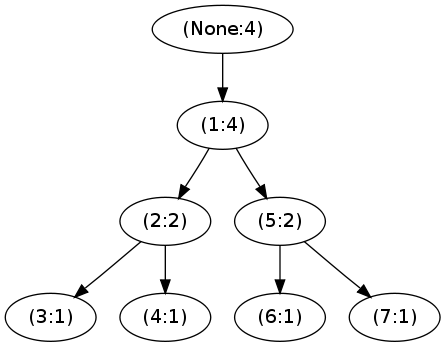
\includegraphics[scale=0.5]{../figs/tiny.png}
\figcaption{The FP-Tree of the full \texttt{tiny.dat} dataset}
\end{center}

Not shown above is a table stored along with the \emph{FP-Tree} which
stores the support of each item in the tree along with a list of nodes
for each item in the tree.

Next, we mine the tree.  If the \emph{FP-Tree} consists of a single
path, then all combinations of frequent items along the path are
frequent patterns.  If the \emph{FP-Tree} has many paths, we go
through each item and build conditional \emph{FP-Trees} of
transactions containing that item, and recursively mining those trees.

\subsection{Eclat}

This algorithm is based around the properties of the vertical data
format, in which each item has an associated transaction id set
(tidset).  The support of an individual item is simply the cardinality
of its tidset.  The support of more than one item is simply the
cardinality of the intersection of the tidsets of the items.

To find all the k-patterns on a dataset, Eclat simply iterates over
all k-combinations of items and for each it checks the cardinality of
the intersection of the items in the combination.  If the cardinality
is at least the minimum support, it reports the pattern.

\begin{center}
\begin{figure*}
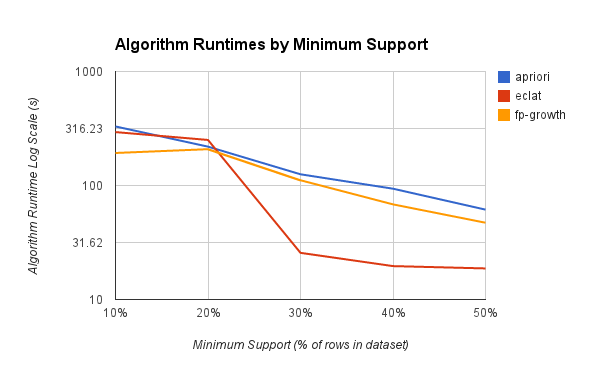
\includegraphics[scale=0.9]{../figs/runtimes_by_min_sup.png}
\caption{Algorithm Runtimes by Minimum Support}
\end{figure*}
\end{center}

\begin{center}
\begin{figure*}
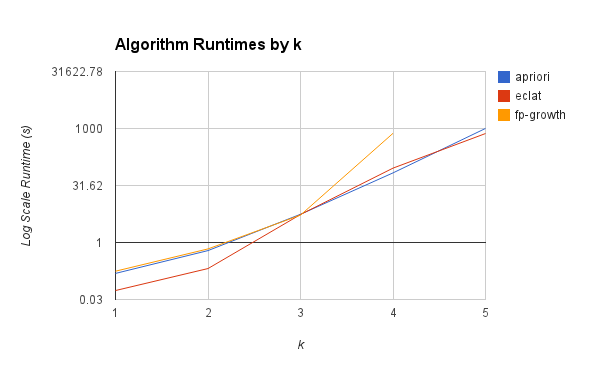
\includegraphics[scale=0.9]{../figs/runtimes_by_k.png}
\caption{Algorithm Runtimes by Length of Pattern (k)}
\end{figure*}
\end{center}

\begin{center}
\begin{figure*}
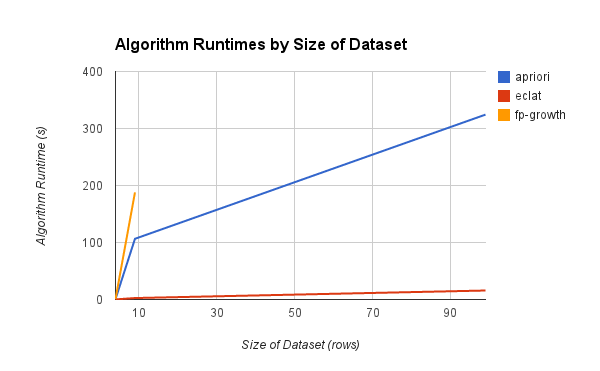
\includegraphics[scale=0.9]{../figs/runtimes_by_rows.png}
\caption{Algorithm Runtimes by Size of Dataset}
\end{figure*}
\end{center}

\section{Testing Methodology}

The various algorithms were tested by measuring the time to find
frequent patterns, varying the independent variables including: the
size of the dataset, the minimum support, and the length of the
desired patterns (k).

\section{Results}
\label{sec:results}

The data show that algorithm runtime gets lower as minimum support gets
higher, gets higher as the length of the patterns increase, and gets
higher as the size of the dataset gets bigger.

More importantly, the \texttt{Eclat} algorithm outperforms
\texttt{Apriori} and \texttt{FP-Growth} when varying dataset size or
minimum support, and remains competitive with \texttt{FP-Growth} for
high values of k, though \texttt{FP-Growth} is best for small
patterns.

Overall, \texttt{Eclat} is the best of the examined algorithms.

\section{Future Work}

One possible direction in which to extend this study is to use the
results of mining datasets for frequent patterns to learn association
rules between items. \cite{wiki_arl}

\appendix
\section{Running Requirements}

To run the code, you simply need to have \texttt{Python 2.6}
installed.  \texttt{Python 2.7} should also work, but the first line
in each python script references \texttt{Python 2.6} in particular,
which should be changed if running on \texttt{Python 2.7}.

There are 4 python scripts included in the code directory:
\texttt{dataset.py}, \texttt{fp\_mining.py}, \texttt{timing.py}, and
\texttt{unit\_tests.py}.

\texttt{dataset.py} simply handles the parsing of files into a simple
datastructure to use for pattern mining.  Running this file with the
name of a datafile as a parameter will run some simple tests on the
module and print the input dataset in its \texttt{Python} format.  The
expected file format is described in the next appendix.

\texttt{fp\_mining.py} containins the algorithm logic for
\texttt{Apriori}, \texttt{FP-Growth}, and \texttt{Eclat}.  The
expected usage of this script is as follows:

\texttt{fp\_mining.py [file] [k] [results]}

Where [file] is the name of an input file, [k] is the desired length
of patterns to mine, and [results] is an optional positive integer
specifying how many results to print.  If [results] is ommitted, all
resulting patterns will be printed.

Note also that this script produces detailed logging output to the
standard error stream on unix, which can be redirected by use of the
\texttt{2>} operator.

\texttt{timing.py} runs the timed tests used to generate the output
discussed in the Results section.  This runs a sequence
of timed tests and prints aggregate information.

\texttt{unit\_tests.py} runs the unit tests for the code base.

\section{Datafile Format}

The datafiles used for testing were retrieved from the FIMI dataset
repository \cite{fimiDatasetRepo}.  The datasets are in a horizontal
format in which each line is an itemset and the items within the set
are integers separated by a single space.  For example, the
hand-written \texttt{tiny.dat} dataset is simply:

\texttt{1 2 3\newline
1 2 4\newline
1 5 6\newline
1 5 7}

The first line is an itemset containing items 1, 2, and 3.  An
important part of the \texttt{Eclat} algorithm is conversion from the
horizontal format to vertical format.

The vertical format of the same data is a dictionary wherein each item
is a key and the value is a \emph{transaction id} set, or
\texttt{tidset}, which contains the IDs of each transaction containing
the key item.

The equivalent vertical format for the \texttt{tiny.dat} dataset is:

\begin{align*}
  1 &: \{ 0, 1, 2, 3 \} \\
  2 &: \{ 0, 1 \} \\
  3 &: \{ 0 \} \\
  4 &: \{ 1 \} \\
  5 &: \{ 2, 3 \} \\
  6 &: \{ 2 \} \\
  7 &: \{ 3 \} \\
\end{align*}

And in \texttt{Python} representation as a dict:

\texttt{\{1:set([0,1,2,3]),2:set([0,1]),3:set([0]),\newline
4:set([1]),5:set([2,3]),6:set([2]),7:set([3])\}}

% Content ends here

\bibliography{references}

\end{multicols} % remove line if you don't want multiple columns
\end{document}
